\section{Koncepce přijímače}
\indent\indent V úvodu bylo uvedeno blokové zapojení ideálního SDR přijímače. Toto zapojení je ale náročné na realizaci, protože vstupní analogově digitální převodník  by musel mít vzorkovací frekvenci minimálně dle Shannonův-Nyquistův-Kotělnikova teorému $f_v > 2f_{max}$. Tedy pro přijímač určený k příjmu pásma 20 metrů by muselo pro vzorkovací frekvenci platit $f_v > 2 \cdot 14,35~MHz$. Takovéto převodníky se sice vyrábějí, ale jejich cena je nad rámec rozpočtu tohoto projektu. Dalším problémem by bylo zpracování objemného datového toku z těchto převodníků. Proto byl  tento koncept analogově digitálního převodníku přímo za anténou zamítnut. Namísto toho byla navržena taková koncepce, která umožňuje výstupní napěťový signál z SDR vzorkovat na prakticky libovolné zvukové kartě s linkovým vstupem.
\begin{figure}[H]
	\centering
	\label{obr:bs_sdr}
	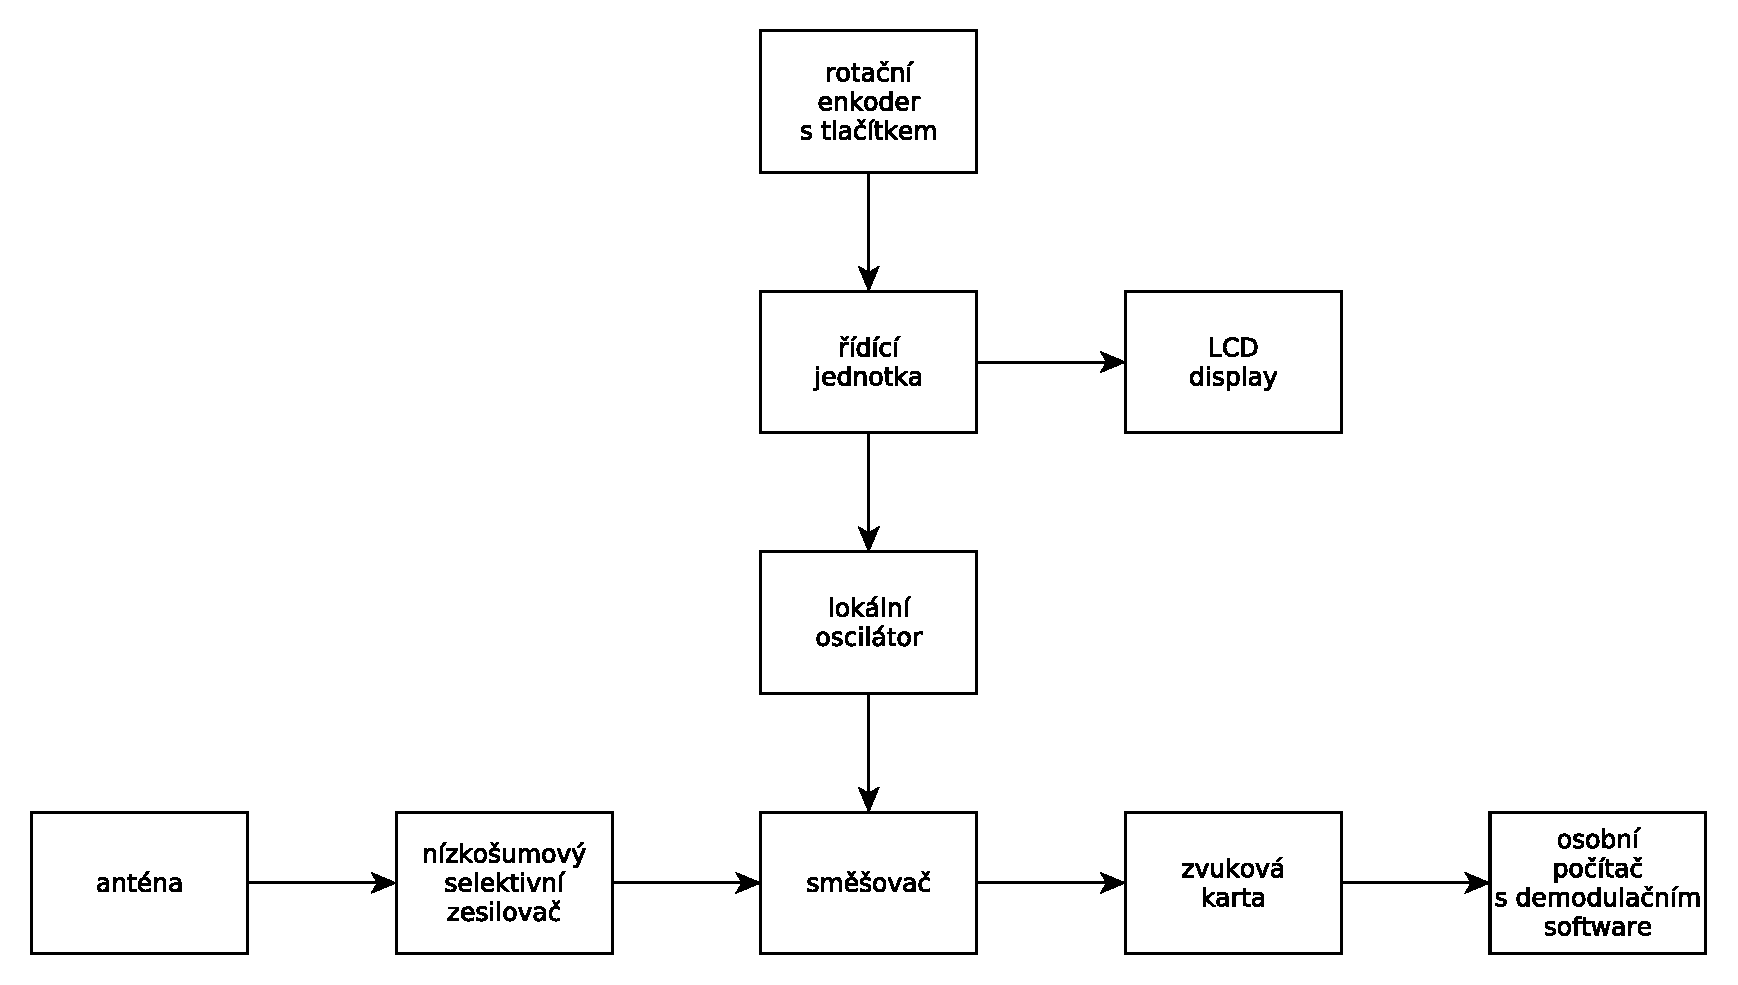
\includegraphics[width=170mm]{img/bs_sdr.pdf}
	\caption{blokové schéma navrženého přijímače}    		
\end{figure}

Toto blokové schéma představuje jednotlivé desky plošných spojů nebo jiných samostatných částí. Tyto bloky budou v následujícím textu postupně rozebírány.





\clearpage